\documentclass{article}
\usepackage[utf8]{inputenc}
% Represent the matrices
\usepackage{amsmath}
% Include images
\usepackage{graphicx}
\graphicspath{ {./images/} }
% Include formatting for code snippets and command line
\usepackage{alltt}
\usepackage{color}
\usepackage{fullpage}
\definecolor{string}{rgb}{0.7,0.0,0.0}
\definecolor{comment}{rgb}{0.13,0.54,0.13}
\definecolor{keyword}{rgb}{0.0,0.0,1.0}

 

\title{Fiducial Marker Detection}
\author{Henrique Poleselo }
\date{January 2019}

\begin{document}

\maketitle

\section{Introduction}
Italic describes a frame.

In ROS:

- Pose is formed by a position (x,y,z) (Point type) which describes a position of a point in free space and an Orientation (x,y,z,w) (Quaternion type) which describes the orientation in free space.

- Transform is formed by a translation (x,y,z) (Vector3 type) which represents a direction in free space and an Orientation (x,y,z,w) (Quaternion type) which describes the orientation in free space as well.

Clarifying a bit about homogeneous transformation matrix (HTM) and its properties. There's a subtle difference between a displacement and pose. And the HTM describes BOTH, the difference being: in case it's a pose, the 3x3 matrix represents the ORIENTATION of the rigid body while de 3x1 vector describes the POSITION. In case it's a displacement then the 3x3 matrix represents the ROTATION between both frames and the 3x1 vector represents the TRANSLATION of the object/frames. In the end the result the same, by doing the transformation between two frames you will get as your "end-pose" a frame, for instance: transforming \textit{world} $\xrightarrow{}$ \textit{end-effector} will result in the end-effector frame.

"The camera pose respect to a marker is the 3d transformation from the marker coordinate system to the camera coordinate system. It is specified by a rotation and a translation vector (see solvePnP() function for more information)." So in order to obtain the DISPLACEMENT of the \textit{camera} wrt. \textit{marker}, we have to to the inverse of it, that means, taking rvec, tvec and then applying a inverse transformation to the rotation and translation matrices.
Note: PnP = Point to Point (2-D to 3-D)
Since we can represent the displacement of rigid body by a 4x4 Matrix:
\[
P=
  \begin{bmatrix}
    R & t \\
    0 & 1
  \end{bmatrix}
\]
Where the R is the rotation matrix (3x3) and t the translation vector (3x1).
Taking the inverse of the Pose is doing the inverse transformation, which is:
\[
P^{-1}=
  \begin{bmatrix}
    R & t \\
    0 & 1
  \end{bmatrix}^{-1}
  =
  \begin{bmatrix}
  -R^T & -R^t*t \\
  0^T & 1
  \end{bmatrix}
\]
* Since the Rotation Matrix is an orthogonal matrix, then it means it’s a square matrix where its transpose is equal to its inverse. Meaning we can spare some efforts by just calculating the transpose instead of the inverse.
See that the normal translation vector has x, y as negative values and z as positive. When inverting the difference is not so big and the x, y change signals to positive. That's because in the inverted perspective the marker reference frame is rotated by 180 degrees around the x-axis, meaning x-y before inverting are flipped (hence, negative), all this considering the standard orientation of the aruco marker, if it was to be rotated, then obviously the signals would be different.
\begin{center}
  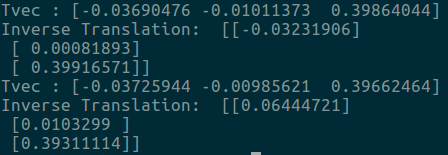
\includegraphics[scale=0.5]{pictures/invertrans.png}
\end{center}

Meaning that the inverse translation and rotation vector we obtain is already the pose of the marker considering the following transformation (from camera to marker). Meaning we should be publishing as a PoseStamped message with the frame-id set to "marker". We then have to rotate it by 180 degrees so our grasping pose could be then correctly oriented.

\section{Betrachtung}

- \textit{marker} $\xrightarrow{}$ \textit{camera} or

- \textit{camera} $\xrightarrow{}$ \textit{marker} 

There’s definitely difference between those transforms. A good way to think about this is: from marker to camera the origin frame (0,0,0) is located where the Marker is and then going to camera (applying translation and rotation). Whereas with camera to marker the origin is located on the camera. 
\\
Some of the cases can be that there’s no difference on the Z-axis regardless the direction of the transformation, like this one:
\begin{center}
  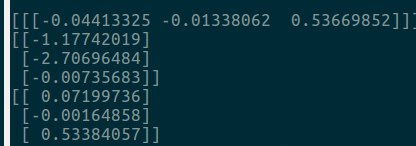
\includegraphics[scale=0.5]{pictures/pic2.jpeg}
  
  Figure 2: Realize that 0.53 is the same after inverting it, which is then 0.53.
\end{center}
Doing the following:
- Take rvec, tvec from estimateMarkerPose
- Do the inversion by inverting the pose matrix
- In the end applying a 180 degree rotation on the x-axis over the inverted pose
- Publish this result in the camera frame to ROS (1)
- Create a broadcaster which transforms the pose received from (1) from camera to marker (hence, creating a tf between the camera and marker).
- After doing all that:
\begin{alltt}
    rosrun tf tf_echo /world /marker 
\end{alltt}
Should return the correct pose of the marker wrt. world. Check the image below: (Figure 3)
\begin{center}
  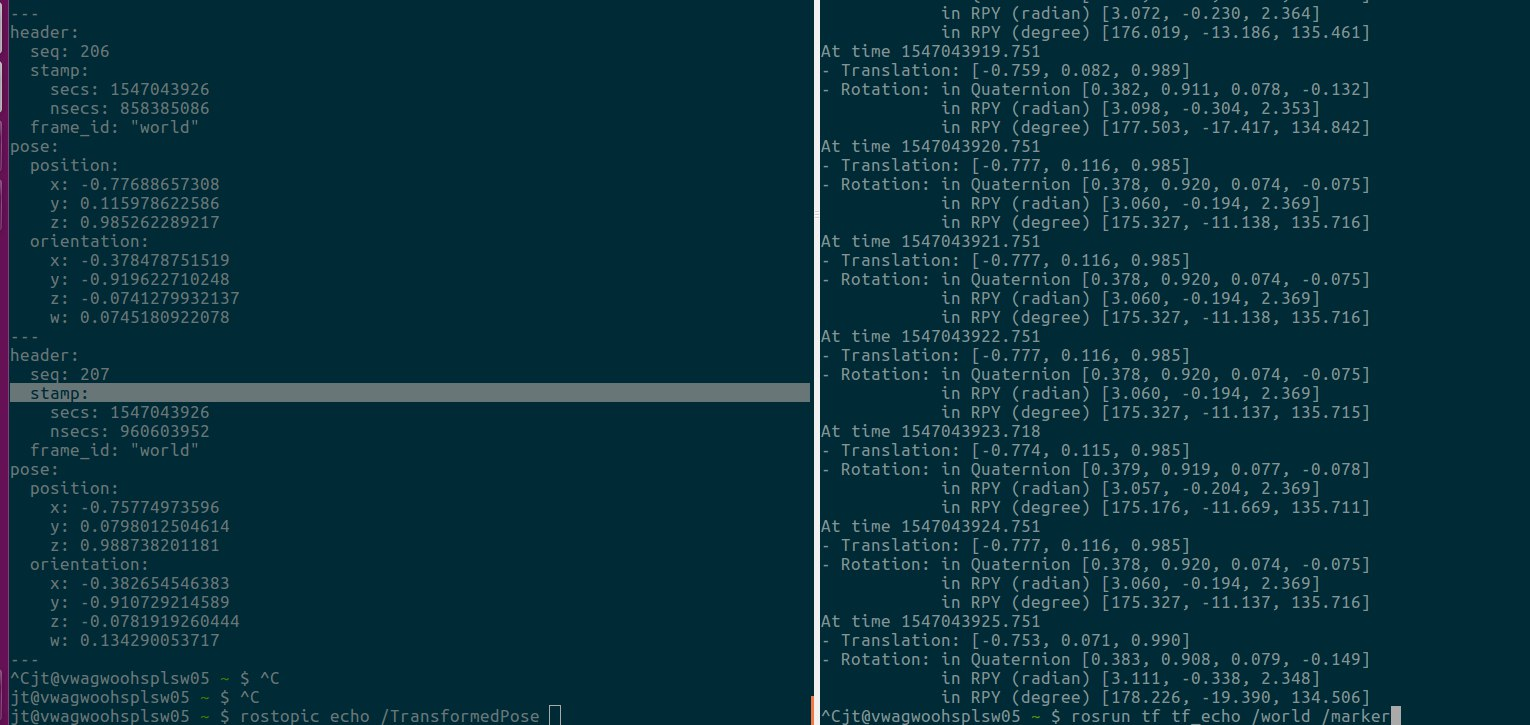
\includegraphics[scale=0.3]{pictures/pic3.jpeg}

  Figure 3:  On the left-hand side is the broadcasted message and right using tf-monitor to check the frames.
\end{center}

\section{Results}
Considering that the TF-Tree is correct and the pose we detect in RVIZ is the same as the pose we are seeing in real life. 
So first things first is by recording the published pose from the topic /AlvarPose1 with aid of rosbag.
\begin{alltt}
    rosbag record /AlvarPose1
\end{alltt}
Then we can convert the ROS messages recorded to .csv format by:
\begin{alltt}
    rostopic echo -b saved_tfd_pose.bag -p /AlvarPose1
\end{alltt}


\section{Filtering Noise}
In case we're not getting the position we are expecting for the robot to grasp the object, we have to somehow debug this, i.e debug the grasping pose. Here are some results obtained from doing the same process as in the section 3.

\begin{center}
    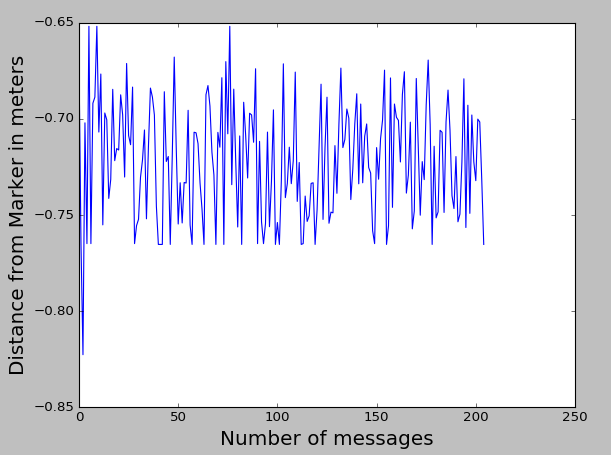
\includegraphics[scale=0.5]{pictures/pic4.png}
    
    Figure 5: X detected values from the /TransformedPose topic
    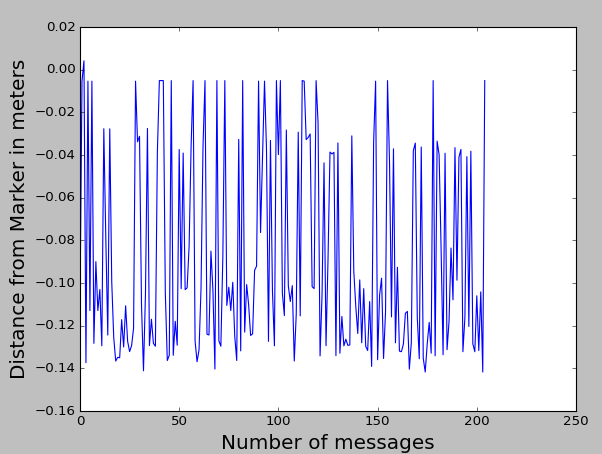
\includegraphics[scale=0.5]{pictures/pic5.png}
    
    Figure 6: Y detected values from the /TransformedPose topic
\end{center}
By extracting the x and y values from the grasp pose we can note a huge noise and applying a Gaussian Filter to both data sets don't bring any good. So we have to see how the data is been captured on the camera, i.e without any transform broadcaster and conversion, because the more operations we apply, more likely to the error to propagate. Therefore we do again the rosbag thing but with /aruco-single/pose which is the detection from the ROS package aruco-single.

\begin{center}
    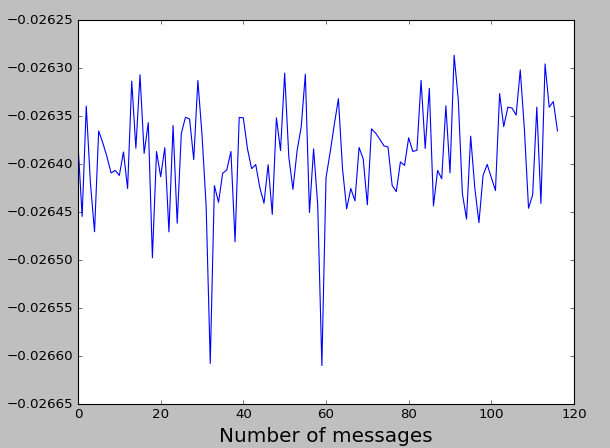
\includegraphics[scale=0.5]{pictures/pic6.png}
    
    Figure 5: X detected values from the /aruco-single/pose topic
    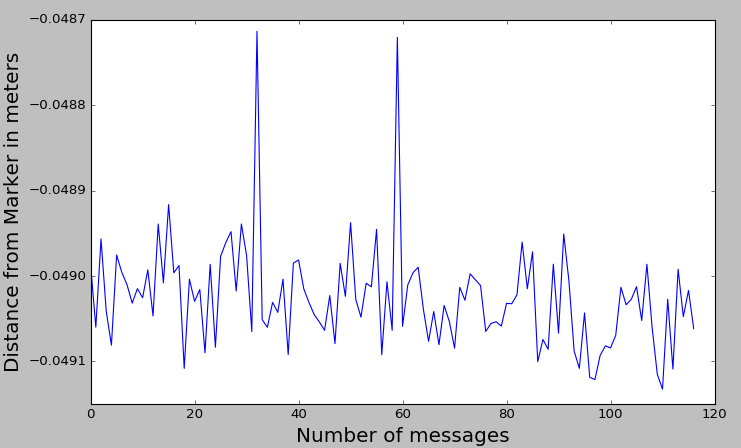
\includegraphics[scale=0.5]{pictures/pic7.png}
    
    Figure 6: Y detected values from the /aruco-single/pose topic
\end{center}
By extracting the x and y values from the file we can see that there's practically no big difference on the detected values, ranging from 0.0488 to 0.0491 or 0.02630 to 0.26660, which for the grasping shouldn't be a big deal.\\
\\
Now, using the detection from a script written in Python.
\begin{center}
    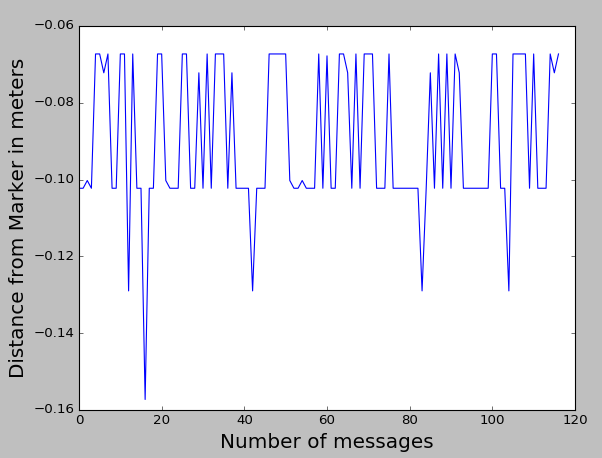
\includegraphics[scale=0.5]{pictures/pic8.png}
    
    Figure 5: X detected values from the /ArucoPose
    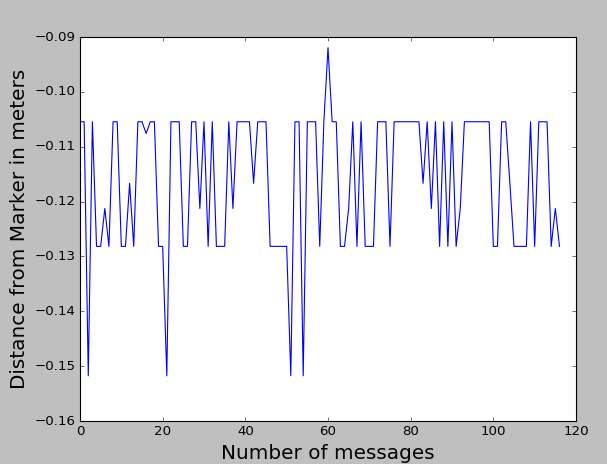
\includegraphics[scale=0.5]{pictures/pic9.png}
    
    Figure 6: Y detected values from the /ArucoPose
\end{center}

Using the same detection but with raw tvec and rvec, without applying any transformation. That means the raw values returned from the method estimateMarkerPose.

\begin{center}
    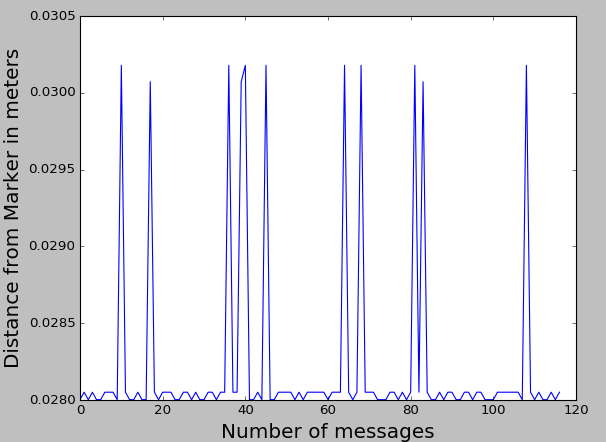
\includegraphics[scale=0.5]{pictures/pic12.png}
    
    Figure 5: X detected values from the /ArucoPose (RAW)
    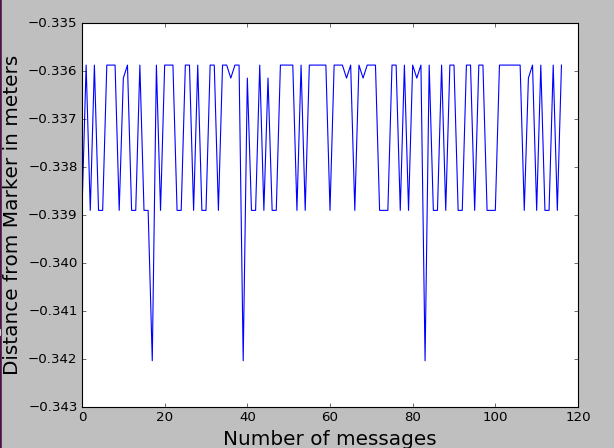
\includegraphics[scale=0.5]{pictures/pic13.png}
    
    Figure 6: Y detected values from the /ArucoPose (RAW)
\end{center}

Applying gaussian filter with sigma = 5 does make a difference, but i don't know yet how good or bad this is.

\begin{center}
    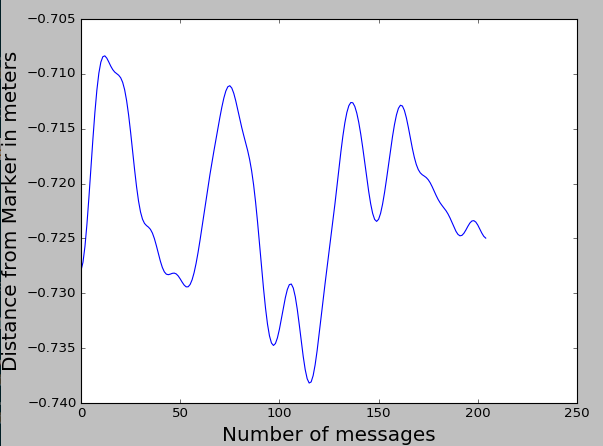
\includegraphics[scale=0.5]{pictures/pic10.png}
    
    Figure 5: Applying Gaussian Filter on /TransformedPose X
    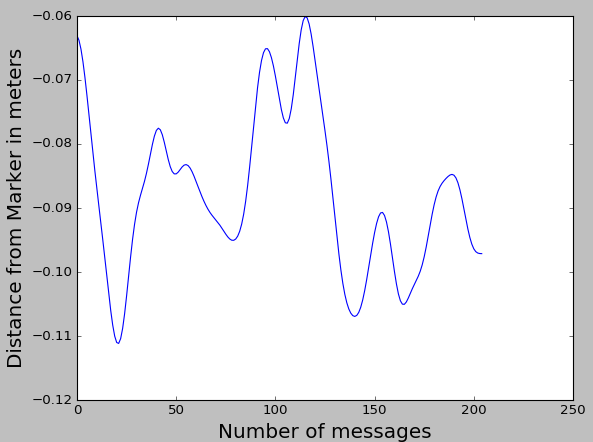
\includegraphics[scale=0.5]{pictures/pic11.png}
    
    Figure 6: Applying Gaussian Filter on /TransformedPose Y
\end{center}

See that the value varies from -0.705 to -0.735 and -0.06 to -0.11. Which gives way more precision around a value, although we KNOW that what we actually want is the value -0.85.

\end{document}
